On Windows operating systems, if you receive an error when starting the application with the message that MSVCP140.dll is missing as shown in \Cref{fig:Missing_CRT_Error}, it is caused by a missing Visual C/C++ runtime library. You can fix this error by running the installer for the Visual C/C++ redistributable package (vc\_redist.x64.exe) which is included with the application.

\begin{figure}[!htbp]
  \centering {
  \softwareSwitch{PBE}{
  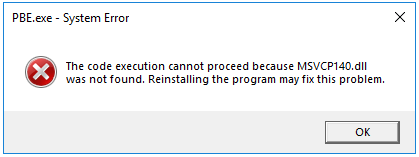
\includegraphics[width=0.8\textwidth]{troubleshooting/figures/PBE-MissingCRT.png}
  }{
  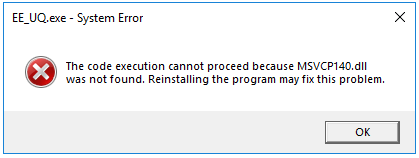
\includegraphics[width=0.8\textwidth]{troubleshooting/figures/EE-UQ-MissingCRT.png} 
  }
  }    
  \caption{Error message for missing Visual C/C++ runtime library}
  \label{fig:Missing_CRT_Error}
\end{figure}

